\chapter{Expérimentations}
	\section{Données}
	\paragraph{}
	Les données de tests sont les même vues dans \ref{part1}\ref{dataSet} aux quelles nous avons rajouté des instances avec plus de variables et plus de clauses pour tester les limites des améliorations apportées par BSO.
	%%Basically same shit as before
	\section{Résultats}
	\subsection{BSO avec paramétrage statique }
	\paragraph{}\label{testconds}
	Nous avons testé notre solveur sur deux types d'instances, \textbf{(u)uf75-325} et \textbf{(u)uf100-430} et \textbf{jnh}\href{http://www.cs.ubc.ca/~hoos/SATLIB/Benchmarks/SAT/DIMACS/JNH/descr.html}{(ici)}, avec un total de dix instances par paramètres et une limite de dix(ou cinq) essaies par instance, les tableaux et figures suivantes montres quels jeux de paramètre ont abouti aux meilleurs résultats durant les test.
		% Please add the following required packages to your document preamble:
		% \usepackage{graphicx}
		\begin{table}[H]
			\resizebox{\textwidth}{!}{%
				\begin{tabular}{|c|c|c|c|c|c|c|c|}
					\hline
					MaxIterations & flip & Nb. d'abeilles & maxChances & Recherches locales & Clauses satis. en moyennes & Taux de satisf. moyen & Temps moyen (s) \\ \hline
					1000 & 5 & 30 & 7 & 15 & 324.72 & 0.9991384615 & 2.65978 \\ \hline
					1000 & 5 & 30 & 9 & 20 & 324.72 & 0.9991384615 & 3.77651 \\ \hline
					1000 & 5 & 30 & 9 & 25 & 324.72 & 0.9991384615 & 4.405 \\ \hline
					1000 & 5 & 30 & 11 & 20 & 324.7 & 0.9990769231 & 3.58024 \\ \hline
					1000 & 5 & 30 & 11 & 30 & 324.7 & 0.9990769231 & 5.73142 \\ \hline
					1000 & 5 & 30 & 7 & 30 & 324.69 & 0.9990461538 & 5.29142 \\ \hline
				\end{tabular}%
			}
			\caption{Meilleures combinaisons des paramètres empiriques pour les instances uf75-325}
			\label{BSO_bestUF}
		\end{table}
	\newpage
	\paragraph{Importance de chaque paramètre}
	Pour mieux se rendre de compte de l'impacte de chaque paramètre, nous avons décidé de fixer chaque valeur d'un paramètre et de faire varier les valeurs des autres paramètres restants et d'en tirer la moyenne, les tableaux suivants résument le travail réalisé :
	
	% Please add the following required packages to your document preamble:
	% \usepackage[table,xcdraw]{xcolor}
	% If you use beamer only pass "xcolor=table" option, i.e. \documentclass[xcolor=table]{beamer}
	\begin{table}[H]
		\centering
		\begin{tabular}{|c|c|}
			\hline
			\textbf{MaxItter}                    & \textbf{Moyenne clauses saisf}.                \\ \hline
			400                         & 324.4436111111                        \\ \hline
			700                         & 324.4419444444                        \\ \hline
			\rowcolor[HTML]{67FD9A} 
			{\color[HTML]{333333} 1000} & {\color[HTML]{333333} 324.4641666667} \\ \hline
		\end{tabular}
		\caption{Impact du paramètres \textbf{MaxItteraitions}}
		\label{average1}
	\end{table}
	% Please add the following required packages to your document preamble:
	% \usepackage[table,xcdraw]{xcolor}
	% If you use beamer only pass "xcolor=table" option, i.e. \documentclass[xcolor=table]{beamer}
	% Please add the following required packages to your document preamble:
	% \usepackage[table,xcdraw]{xcolor}
	% If you use beamer only pass "xcolor=table" option, i.e. \documentclass[xcolor=table]{beamer}
	\begin{table}[H]
		\centering
		\begin{tabular}{|c|c|}
			\hline
			\textbf{flip} & \textbf{Moyenne clauses saisf.} \\ \hline
			\rowcolor[HTML]{67FD9A} 
			5    & 324.4247222222         \\ \hline
			7    & 324.4419444444         \\ \hline
			9    & 324.4641666667         \\ \hline
		\end{tabular}
		\caption{Impact du paramètres \textbf{Flip}}
		\label{average2}
	\end{table}
	
	
	% Please add the following required packages to your document preamble:
	% \usepackage[table,xcdraw]{xcolor}
	% If you use beamer only pass "xcolor=table" option, i.e. \documentclass[xcolor=table]{beamer}
	\begin{table}[H]
		\centering
		
		\begin{tabular}{|c|c|}
			\hline
			\textbf{nbr abeilles} & \textbf{Moyenne clauses saisf.} \\ \hline
			\rowcolor[HTML]{67FD9A} 
			7            & 324.4641666667         \\ \hline
			9            & 324.4419444444         \\ \hline
			11           & 324.4247222222         \\ \hline
		\end{tabular}
		\caption{Impact du paramètres \textbf{Nombre d'abeilles}}
		\label{average3}
	\end{table}
	
	
	% Please add the following required packages to your document preamble:
	% \usepackage{graphicx}
	% \usepackage[table,xcdraw]{xcolor}
	% If you use beamer only pass "xcolor=table" option, i.e. \documentclass[xcolor=table]{beamer}
	\begin{table}[H]
		\centering
			\begin{tabular}{|c|c|}
				\hline
				\textbf{recherches locales} & \textbf{Moyenne clauses saisf.} \\ \hline
				15                          & 324.4251851852                  \\ \hline
				20                          & 324.4248148148                  \\ \hline
				\rowcolor[HTML]{67FD9A} 
				25                          & 324.4644444444                  \\ \hline
				30                          & 324.46                          \\ \hline
			\end{tabular}%
		
		\caption{Impact du paramètres \textbf{Nombre de recherches locales}}
		\label{average4}
	\end{table}
	
	\subsection{BSO avec paramétrage dynamique }
	\subsubsection{Traitement non-parallèle}
	\paragraph{}
	Après avoir améliorer le choix des paramètres, en le rendant dynamique et dépendant de l'exécution courante, nous avons obtenus de bien meilleures résultats, non seulement sur les même instances mais aussi sur d'autres de nature beaucoup plus complexe, les conditions sont toujours les mêmes voir \ref{testconds}
	\begin{table}[H]
		\centering
		
		\begin{tabular}{|c|c|c|c|}
			\hline
			\textbf{Instance} & \textbf{clauses sais.} & \textbf{Taux} & \textbf{Temps(s)} \\ \hline
			uf75-01           & 325                    & 1             & 1.5592            \\ \hline
			uf75-02           & 325                    & 1             & 2.0478            \\ \hline
			uf75-03           & 325                    & 1             & 8.4525            \\ \hline
			uf75-04           & 324.9                  & 0.9996923077  & 11.878            \\ \hline
			uf75-05           & 325                    & 1             & 7.8659            \\ \hline
			uf75-06           & 325                    & 1             & 6.1555            \\ \hline
			uf75-07           & 325                    & 1             & 6.3884            \\ \hline
			uf75-08           & 325                    & 1             & 6.0486            \\ \hline
			uf75-09           & 325                    & 1             & 2.4297            \\ \hline
			uf75-010          & 325                    & 1             & 1.7065            \\ \hline
			Moyenne           & 324.99                 & 0.9999692308  & 5.45321           \\ \hline
		\end{tabular}
		\caption{Résume pour les instances \textbf{uf75-325}}
	\end{table}
	
	
	
	\begin{table}[H]
		\centering
		\begin{tabular}{|c|c|c|c|}
			\hline
			\textbf{instance} & \textbf{clauses satis.} & \textbf{Taux} & \textbf{Temps(s)} \\ \hline
			uf100-01          & 430                        & 1             & 25.8205       \\ \hline
			uf100-02          & 429.6                      & 0.9990697674  & 49.4153       \\ \hline
			uf100-03          & 430                        & 1             & 19.8098       \\ \hline
			uf100-04          & 430                        & 1             & 11.4756       \\ \hline
			uf100-05          & 429.9                      & 0.9997674419  & 36.687        \\ \hline
			uf100-06          & 430                        & 1             & 2.0742        \\ \hline
			uf100-07          & 430                        & 1             & 9.2083        \\ \hline
			uf100-08          & 429.4                      & 0.9986046512  & 56.0873       \\ \hline
			uf100-09          & 430                        & 1             & 14.9025       \\ \hline
			uf100-010         & 430                        & 1             & 18.9783       \\ \hline
			Moyenne           & 429.89                     & 0.999744186   & 24.44588      \\ \hline
		\end{tabular}
		\caption{Résume pour les instances \textbf{uf100-430}}
		\label{my-label}
	\end{table}
	
	\begin{table}[H]
		\centering
		\begin{tabular}{|c|c|c|c|}
			\hline
			\textbf{instance} & \textbf{clauses satis.} & \textbf{Taux} & \textbf{Temps(s)} \\ \hline
			jnh201            & 800                        & 1             & 11.704        \\ \hline
			jnh202            & 798.8                      & 0.9985        & 82.441        \\ \hline
			jnh203            & 798.8                      & 0.9985        & 81.8918       \\ \hline
			jnh204            & 800                        & 1             & 40.7106       \\ \hline
			jnh205            & 800                        & 1             & 34.9264       \\ \hline
			Moyenne           & 799.52                     & 0.9994        & 50.33476      \\ \hline
		\end{tabular}
		\caption{Résume pour les instances \textbf{jnh200-800}}
	\end{table}
	
	\newpage
	
	\paragraph{}
	Pour illustrer l'importance de cette modification, la figure suivante montre le taux de satisfiabilité selon la taille du problème(nombre de variables/de clauses) : 
	\begin{figure}[H]
		\centering
		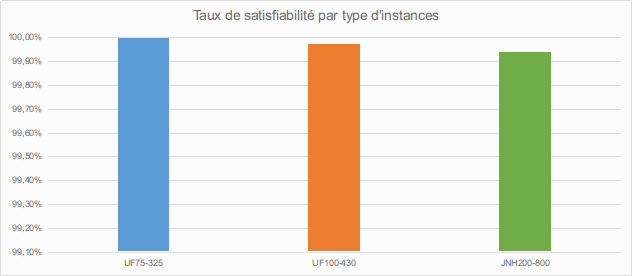
\includegraphics[width=\textwidth]{images/uf75_uf100_jnh200.png}
		\caption{Taux de satisfiabilité selon la nature de l'instance}
	\end{figure}
	
	\subsubsection{Traitement parallèle}
	\paragraph{}
	Nous avons décidé de tenter une approche parallèle à la résolution du problème, en considérant chaque abeille comme un thread pouvant réaliser son travail indépendamment des autres abeilles, les résultats en terme de taux de satisfiabilité n'ont pas beaucoup changé, mais une nette amélioration du temps d'exécution peut être soulignée, le graphe et le tableau suivants comparent les deux technique(parallèle vs non-parallèle) en terme de ce dernier : 
	\begin{table}[H]
		\centering
		\caption{My caption}
		\label{my-label}
		\begin{tabular}{|c|c|c|c|c|c|}
			\hline
			\textbf{UF75-325} & \textbf{UF75-325 PAR} & \textbf{UF100-430} & \textbf{UF100-430 PAR} & \textbf{JNH200-800} & \textbf{JNH200-800 PAR} \\ \hline
			5,45321           & 2,27845               & 24,44588           & 13,01019               & 312,4600            & 50,3348                 \\ \hline
		\end{tabular}
	\end{table}
	\begin{figure}[H]
		\centering
		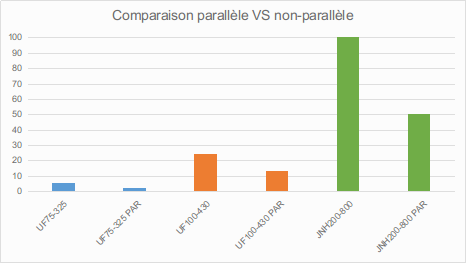
\includegraphics[width=\textwidth]{images/parVSnonPar.png}
		\caption{Apport du parallélisme}
	\end{figure}
	\section{Comparaison avec les méthodes de \ref{part1}}
	\paragraph{}
	Il est évident que l'approche vu dans cette partie surpasse de loin celle vu en partie \ref{part1}, là oû la meilleure des méthodes constructives (A*) ne donnait pas de bon résultats, l'algorithme BSO lui y est clairement un  supérieur, que ce soit en terme d'exactitude ou d'exploitation de ressources(i.e mémoire et temps d'exécution). N'est en moins, cette algorithme admet des limites, et sa nature stochastique n'en fait pas une méthode fiables a 100\%( risque de stagnation prématurée, optimum local, réglage des paramètres couteux en temps .. ), cela nous a amené a explorer un autre algorithme de la même famille(métaheuristiques) mais qui exploite l'approche de construction de solution en même temps, notre choix s'est porté sur ACO (Ant Colony Optimization).
	%talk about how BSO is amazing
